%%%%%%%%%%%%%%%%%%%%%%%%%%%%%%%%%%%%%%%%%%%%%%%%%%%%%%%%%%%%%%%%%%
%                           Document style
%%%%%%%%%%%%%%%%%%%%%%%%%%%%%%%%%%%%%%%%%%%%%%%%%%%%%%%%%%%%%%%%%%
\documentclass[12pt]{article}

% Importing report style and the first pages 
%%%%%%%%%%%%%%%%%%%%%%%%%%%%%%%%%%%%%%%%%%%%%%%%%%%%%%%%%%%%%%%%%%
%                       Main document style 
%%%%%%%%%%%%%%%%%%%%%%%%%%%%%%%%%%%%%%%%%%%%%%%%%%%%%%%%%%%%%%%%%%

% Importing user packages (librarys for different functions and commands) 
\usepackage[utf8]{inputenc}         % interprets charecters as if they comply to ASCII standards
\usepackage{todonotes}              % to do notes 
\usepackage{subfiles}               % add subfiles
\usepackage[T1]{fontenc}            % text font
\usepackage{lmodern}                % font
\usepackage{pdfpages, pdflscape}    % add pdf's 
\usepackage{gensymb, textcomp}      % add symbols
\usepackage{lastpage}               % get the last page number 
\usepackage{graphicx}               % add images 
\usepackage{tabularx}               % add tables 
\usepackage{mathtools}              % math
\usepackage{listings}               % add lists (code)
\usepackage{enumitem}               % options for enumerate
\usepackage{setspace}               % define size of space (infinite) 
\usepackage{xcolor}                 % colors
\usepackage{fancyhdr}               % to get fancy headers
\usepackage [background=black, arrow=red, text=white]{callouts}      % add callouts 
\usepackage{wrapfig}                % positioning figures
\usepackage{subcaption}             % position mulitple figures 
\usepackage{tikz}
\usepackage{upquote}
\usepackage{tikz}                   % text on top of images
\usepackage[document]{ragged2e}
\usepackage{float}

% page settings
\setlength{\marginparwidth}{2cm}    % margins
\usepackage[a4paper,left=2.5cm,right=2.5cm,top=2.5cm,bottom=4cm]{geometry}                 % dimensions 
\setlength\parindent{0pt}
\setlength{\parskip}{1em}

\renewcommand{\contentsname}{Contents} % content table 

\setlength{\headheight}{35.372pt} % header height

\cfoot\thepage % page number as footer

% creating base header 
\pagestyle{fancy}
% \rhead{\includegraphics[width=3.2cm]{images/ntnu_logo.png}}
\rhead{z3531215}

%define colors for links
\definecolor{ceruleanblue}{rgb}{0.16, 0.32, 0.75}
\definecolor{coolblack}{rgb}{0.0, 0.18, 0.39}


% clickable table of contents
\usepackage{hyperref}
\hypersetup{linktoc = all, colorlinks=true, linkcolor=coolblack, filecolor=magenta, urlcolor=ceruleanblue, citecolor=ceruleanblue}

% number of subsections in table of contents
\setcounter{tocdepth}{4}
\setcounter{secnumdepth}{4}


% defining code types
% CSS
\lstdefinelanguage{CSS}{
  keywords={color,background-image:,margin,padding,font,weight,display,position,top,left,right,bottom,list,style,border,size,white,space,min,width, transition:, transform:, transition-property, transition-duration, transition-timing-function},	
  sensitive=true,
  morecomment=[l]{//},
  morecomment=[s]{/*}{*/},
  morestring=[b]',
  morestring=[b]",
  alsoletter={:},
  alsodigit={-}
}

% JavaScript
\lstdefinelanguage{JavaScript}{
  morekeywords={typeof, new, true, false, catch, function, return, null, catch, switch, var, if, in, while, do, else, case, break},
  morecomment=[s]{/*}{*/},
  morecomment=[l]//,
  morestring=[b]",
  morestring=[b]'
}

\lstdefinelanguage{HTML5}{
  language=html,
  sensitive=true,	
  alsoletter={<>=-},	
  morecomment=[s]{<!-}{-->},
  tag=[s],
  otherkeywords={
  % General
  >,
  % Standard tags
	<!DOCTYPE,
  </html, <html, <head, <title, </title, <style, </style, <link, </head, <meta, />,
	% body
	</body, <body,
	% Divs
	</div, <div, </div>, 
	% Paragraphs
	</p, <p, </p>,
	% scripts
	</script, <script,
  % More tags...
  <canvas, /canvas>, <svg, <rect, <animateTransform, </rect>, </svg>, <video, <source, <iframe, </iframe>, </video>, <image, </image>, <header, </header, <article, </article, <h1, </h1, <h2, </h2
  },
  ndkeywords={
  % General
  =,
  % HTML attributes
  charset=, src=, id=, width=, height=, style=, type=, rel=, href=, class=, name=, content=, lang=,
  % SVG attributes
  fill=, attributeName=, begin=, dur=, from=, to=, poster=, controls=, x=, y=, repeatCount=, xlink:href=,
  % properties
  margin:, padding:, background-image:, border:, top:, left:, position:, width:, height:, margin-top:, margin-bottom:, font-size:, line-height:, display:, font-family:, 
  background-color:,
	% CSS3 properties
  transform:, -moz-transform:, -webkit-transform:,
  animation:, -webkit-animation:,
  transition:,  transition-duration:, transition-property:, transition-timing-function:,
  }
}

\lstdefinestyle{htmlcssjs} {%
  % General design
%  backgroundcolor=\color{editorGray},
  basicstyle={\footnotesize\ttfamily},   
  frame=b,
  % line-numbers
  xleftmargin={0.75cm},
  numbers=left,
  stepnumber=1,
  firstnumber=1,
  numberfirstline=true,	
  % Code design
  identifierstyle=\color{black},
  keywordstyle=\color{blue}\bfseries,
  ndkeywordstyle=\color{editorGreen}\bfseries,
  stringstyle=\color{editorOcher}\ttfamily,
  commentstyle=\color{brown}\ttfamily,
  % Code
  language=HTML5,
  alsolanguage=JavaScript,
  alsodigit={.:;},	
  tabsize=2,
  showtabs=false,
  showspaces=false,
  showstringspaces=false,
  extendedchars=true,
  breaklines=true,
  % German umlauts
  literate=%
  {Ö}{{\"O}}1
  {Ä}{{\"A}}1
  {Ü}{{\"U}}1
  {ß}{{\ss}}1
  {ü}{{\"u}}1
  {ä}{{\"a}}1
  {ö}{{\"o}}1
}


%%%%%%%%%%%%%%%%%%%%%%%%%%%%%%%%%%%%%%%%%%%%%%%%%%%%%%%%%%%%%%%%%%
%                   Command for the first page 
%%%%%%%%%%%%%%%%%%%%%%%%%%%%%%%%%%%%%%%%%%%%%%%%%%%%%%%%%%%%%%%%%%

\newcommand*\FirstPage{
\thispagestyle{empty}
    \raggedleft % Right align the title page
	
	\rule{1pt}{\textheight} % Vertical line
	\hspace{0.05\textwidth} % Whitespace between the vertical line and title page text
	\parbox[b]{0.75\textwidth}{ % Paragraph box for holding the title page text, adjust the width to move the title page left or right on the page
		
		{\Huge\bfseries ZEIT8219 \\[0.4\baselineskip] Satellite Communications }\\[2\baselineskip] % Title
		{\large\textit{Assignment 1}}\\[4\baselineskip] % Subtitle or further description
		{\Large\textsc{Nina Averill}}\\[0.5\baselineskip] % Author name, lower case for consistent small caps
		{\large\text{z3531215}}
		
		\vspace{0.5\textheight} % Whitespace between the title block and the publisher
		
		{\noindent UNSW Canberra}\\[0.3\baselineskip] 
		{\noindent Apr 2022}\\[\baselineskip] % Publisher and logo
	}
    
}



%%%%%%%%%%%%%%%%%%%%%%%%%%%%%%%%%%%%%%%%%%%%%%%%%%%%%%%%%%%%%%%%%%
%                   Command for the second page
%%%%%%%%%%%%%%%%%%%%%%%%%%%%%%%%%%%%%%%%%%%%%%%%%%%%%%%%%%%%%%%%%%

\newcommand*\SecondPage{
\thispagestyle{fancy}

% creating base header 
% \rhead{\includegraphics[width=3.2cm]{images/ntnu_logo.png}}

% section header
\lhead{Prosjektoppgave Vår 2020}

% recreating the table from the given Word-report-template
\begin{table}[ht]
\setlength\extrarowheight{5pt}
    
    % first row
    \begin{tabularx}{\textwidth}{|X|}
        \hline
        \textbf{KANDIDATER (etternavn, fornavn):} \newpara
        Navn
    \end{tabularx}
    
    % second row
    \begin{tabularx}{\textwidth}{|p{1,4cm}|p{2,4cm}|p{4,4cm}|p{4,2cm}|p{2,25cm}|}
    \hline
    \textbf{DATO:} & \textbf{FAGKODE:} & \textbf{GRUPPE (navn/nr):} & \multicolumn{1}{c|}{\textbf{SIDER/BILAG:}} & \textbf{BIBL. NR:}\\
    30.04.20 & TST101 & \multicolumn{1}{c|}{Team Pro / Gruppe 16} & \multicolumn{1}{c|}{\pageref{LastPage} / 8} & N/A \\ 
    \hline
    \end{tabularx}
    
    % third row
    \begin{tabularx}{\textwidth}{|X|}
        \textbf{FAGLÆRER(E):} \\
        Navn \\
        \hline
    \end{tabularx}
    
    % forth row
    \begin{tabularx}{\textwidth}{|X|}
        \textbf{TITTEL:} \\
        Tittel \\
        \hline
    \end{tabularx}
    
    %fifth row
    \begin{tabularx}{\textwidth}{|X|}
        \addSammendrag \\ % new command to at the text file from sections (more orginised to write this way)
        \hline
    \end{tabularx}
\end{table}}



%%%%%%%%%%%%%%%%%%%%%%%%%%%%%%%%%%%%%%%%%%%%%%%%%%%%%%%%%%%%%%%%%%
%                       New Commands
%%%%%%%%%%%%%%%%%%%%%%%%%%%%%%%%%%%%%%%%%%%%%%%%%%%%%%%%%%%%%%%%%%

%creating paragraphs --> \newpara
\newcommand{\newpara}{\vskip 2mm}

%add pdf's --> \addpdf
\newcommand*\addpdf[1]{
\includepdf[pages=-]{#1}}

%add pdf's in landscape --> \addpdflandscape
\newcommand*\addpdflscape[1]{
\begin{landscape}
\newgeometry{margin=0cm}
\includepdf[pages=-,angle=90]{#1}
\end{landscape}} 

%add conclusion (used in second-page table) --> \addSammendrag
% \newcommand*\addSammendrag{
% \subfile{sections/00_sammendrag.tex}}

%add sections with 4 numbers --> \paragraph
\usepackage{titlesec}
\setcounter{secnumdepth}{4}
\titleformat{\paragraph}
{\normalfont\normalsize\bfseries}{\theparagraph}{1em}{}
\titlespacing*{\paragraph}
{0pt}{3.25ex plus 1ex minus .2ex}{1.5ex plus .2ex}

\definecolor{codegray}{RGB}{242, 242, 242}
\definecolor{codegreen}{RGB}{57, 172, 115}
\lstdefinestyle{mystyle}{
    backgroundcolor=\color{codegray},   
    commentstyle=\color{codegreen},
    basicstyle=\ttfamily\footnotesize,
    breakatwhitespace=false,         
    breaklines=true,
    postbreak=\mbox{\textcolor{codegreen}{$\hookrightarrow$}\space},
    captionpos=b,                    
    keepspaces=true,                 
    numbers=left,                    
    numbersep=5pt,                  
    showspaces=false,                
    showstringspaces=false,
    showtabs=false,                  
    tabsize=4
}
\lstset{style=mystyle}

% sections without numbers, but still in table of contents
%\setcounter{secnumdepth}{0} % remove "%" to include


%=================================================================
%                           Summary
%=================================================================
\begin{document}

% adding the first two pages 
\FirstPage
% \SecondPage
\pagebreak

% creating table of contents 
\setlength{\parskip}{0em}
\lhead{Contents} % section header
\renewcommand{\baselinestretch}{0.95}\normalsize
\tableofcontents
\renewcommand{\baselinestretch}{1.0}\normalsize
\setlength{\parskip}{1em}
\newpage

% adding the different sections
\section{Report Summary}
\lhead{Summary} % section header

\raggedright

This report will outline a constellation of three inclined geosynchronous satellites designed to provide continuous coverage of mainland Australia, Tasmania and various remote offshore territories. The locations of the remote offshore territories are described below:

\begin{table}[H]
\begin{tabular}{lll}
 \hline
Remote Territory                  & Latitude (deg) & Longitude (deg) \\
Ashmore Island                    & 12°11'S        & 122°59'E        \\
Cartier Island                    & 12°31'S        & 123°33'E        \\
Casey Research Station            & 66°17'S        & 110°32'E        \\
Davis Research Station            & 68°35'S        & 77°58'E         \\
Mawson Research Station           & 67°36'S        & 62°52'E         \\
Macquarie Island Research Station & 54°30'S        & 158°57'E        \\
Christmas Island                  & 10°25'S        & 105°43'E        \\
Cocos (Keeling) Island            & 12°10'S        & 96°50'E         \\
Coral Sea Islands                 & 23°15'S        & 155°32'E        \\
Heard \& McDonald Islands         & 53°05'S        & 73°30'E         \\
Norfolk Island                    & 29°02'S        & 167°57'E       \\  \hline
\end{tabular}
\caption{Remote Offshore Territories locations in Geographic Coordinates}
\label{table:remote_offshore}
\end{table}

In the following, we will define the constellation of satellites, as well as provide proof of coverage and perform a minimal link analysis for three of the remote offshore territories. For the purposes of this analysis we will assume a spherical Earth with radius equal to 6371 km and no orbital perturbations, i.e. gravitational attraction is the only force acting on the satellite. 

GMAT is the primary tool used for orbit propagation and visualisation, as well as coordinate transformation. All equations can be assumed to be sourced from Principles of Satellite Communications (Ryan, 2021) unless stated otherwise.

\newpage
%=================================================================
%                           Constellation
%=================================================================
\section{Satellite Constellation}
\lhead{Satellite Constellation} % section header
\raggedright
\subsection{Definition}
To guarantee continuous coverage for all of Australia and its offshore territories, we defined a constellation of three inclined geosynchronous satellites. The Keplerian orbital parameters  of the constellation in the J2000 inertial reference frame are defined in Table \ref{table:orbital_params}.

\begin{table}[h]
\begin{tabular}{lllllll}
 \hline
\begin{tabular}[c]{} Satellite \\ name \end{tabular}   & \begin{tabular}[c]{} Semi-major \\ axis \\ (km)\end{tabular} & \begin{tabular}[c]{} Eccen- \\ tricity\end{tabular}  & \begin{tabular}[c]{} Inclination \\ (deg) \end{tabular}   & \begin{tabular}[c]{@{}l@{}}Right ascension\\  of the ascending \\  node (deg)\end{tabular} & \begin{tabular}[c]{} Argument of \\ perigee \\ (deg) \end{tabular}   & \begin{tabular}[c]{} True  \\ Anomaly \\ (deg) \end{tabular}\\  \hline
COMMSAT1       & 42165                & 0            & 30                & 30                                                                                        & 0                         & 0                  \\
COMMSAT2       & 42164                & 0            & 30                & 150                                                                                       & 0                         & 240                \\
COMMSAT3       & 42165                & 0            & 30                & 270                                                                                       & 0                         & 120      \\  \hline         
\end{tabular}
\caption{Keplerian orbital parameters of the constellation in the J2000 inertial coordinate system  }
\label{table:orbital_params}
\end{table}

The semi-major axis and eccentricity were specified such that the orbital period is equal to the length of the sidereal day, defining the orbital regime as geo-synchronous. An inclined orbit increases the north-south ground trace, ensuring coverage for the southernmost Earth stations. A constellation of three satellites ensured that there was always a satellite in view of the Earth stations, and there is no risk of collision at the point of intersection of the orbits. The right ascension of the ascending node and true anomaly are offset such that the satellites had to be equally placed in the ground trace, which is located roughly in the centre of the span of coverage.

Given these initial orbital parameters, GMAT was used to propagate the orbit for a full sidereal day from the UTC datetime 01 Jan 2000 11:59:28.000 [\ref{code:gmat}]. Figures \ref{fig:j2000_xy} and \ref{fig:j2000_ecliptic}  show the orbits of the constellation with respect to the J2000 inertial frame defined above, displaying the X-Y and ecliptic planes respectively. Figures \ref{fig:fixed_xy} and \ref{fig:fixed_ecliptic}  further show the orbits with respect to an earth-fixed reference frame, displaying the X-Y and ecliptic planes respectively. 

\subsection{Technical Reasoning}
The constellation of inclined geosynchronous orbits was selected as it met the minimal criteria of continuous coverage of all of the mainland and remote ground stations. The broad benefit of this orbital height is that it provides a large coverage area relative to the number of satellites in the constellation. This orbit has a number of benefits and implications that will be explored below.  

\subsubsection{Launch Costs}
    The orbit regime selected will require a launch inclination greater than the minimum orbital inclination. At thirty degrees inclination, there are a number of launch sites where this is possible. Therefore, the satellite will have to perform a smaller, and therefore less expensive, plane change manoeuvre than most geostationary launches. However, the satellites will still have to perform a geostationary transfer orbit to reach the final parking orbit. The greater fuel (and therefore weight) requirements will incur additional launch costs than a comparable Lower Earth Orbit (LEO) constellation.  
    
\subsubsection{Satellite Costs}
    Geosynchronous Equatorial Orbit (GEO) satellites tend to be more expensive to develop due to their increased size and system complexity compared to LEO and Medium Earth Orbit (MEO) constellations. However, this comes with the benefit of a reduced number of satellites in the constellation required to provide the same area of coverage.  

\subsubsection{Satellite Lifespan}
    Satellites in the geostationary orbit tend to have much greater mission lifespans than lower orbits, with most missions planning for around fifteen year life-spans. The main limitations on the satellite's lifetime is the fuel requirements for station-keeping and disposal, and the degradation of on-board systems from the harsh radiation environment. Lower orbit regimes generally have a much shorter lifespan of 7-10 years, with the main limitation being orbit deterioration as a result of atmospheric drag. 

\subsubsection{Ground Infrastructure complexity and costs}
    Geosynchronous orbits tend to have less complex ground station requirements as remain effectively stationary with respect to the Earth. However as the orbit regime chosen has a significantly inclined orbit, the ground track traces a figure-eight path and the ground stations will need to have some tracking capabilities. Moreover, the large propagation distance will lead to greater requirements for high-power transmitters, sensitive receivers and high-gain antennas at the ground station. 

\subsubsection{Service Availability}
    The main risks to service availability for the geo-inclined orbits come from solar interference, and solar eclipses from the Earth and the Moon. Sun-transit outages occur when the beam of the ground station antenna is pointed directly at the sun, with the broad-spectrum radio frequency energy emitted from the sun causing disruption to the receive signal. As seen in Figures \ref{fig:j2000_ecliptic} and \ref{fig:fixed_ecliptic}, the Earth's ecliptic plane intersects with the orbital plane of the satellite and so there is some significant risk of interference. Geo-synchronous orbits tend to experience less frequent Earth and Lunar eclipses than lower orbits, but precautionary measures still need to be taken to ensure that the satellites have access to backup power sources, or reduced service capabilities during the eclipse period.

\subsubsection{Coverage Extent}
    The constellation meets the minimal requirement for continuous coverage for all ground stations. In addition to this, Figure \ref{fig:cocos_elevation}, \ref{fig:norfolk_elevation}, and \ref{fig:mawson_elevation} indicate that there is often multiple satellites in view at any one moment, this provides additional redundancy in case one satellite in the constellation is experiencing an outage. 

\subsubsection{Latency}
    Due to the greater orbital height, geo-synchronous satellites have significantly greater latency than lower orbit regimes. The minimum time taken for a communication round trip is around 250 ms, making it ineffective for some communication protocols that require near real-time interactions.


%=================================================================
%                           Coverage
%=================================================================
\section{Ground Station Link Analysis}
\lhead{Coverage} % section header

\subsection{Coverage}
A best-case analysis of the ground station coverage was conducted for the Cocos Islands, Mawson Research Station and Norfolk Island. To evaluate the optimal point in the satellites' orbit, the minimum slant range was calculated with respect to each ground station. Slant range is generally considered to be a good indicator of the quality of communication as a smaller propagation distance generally indicates less path attenuation. 

As all three satellites trace the same path and have the same transmit characteristics, each would exhibit the same link behaviour with each ground station over the course of the orbit. The optimal link characteristic were therefore calculated with reference to COMMSAT1, but equivalent values could be found with reference to COMMSAT2 and COMMSAT3. 

GMAT was used to propagate the orbits over the course of a sidereal day and output the latitude and longitude of the sub-satellite point and orbital radius for each time step. Equation \ref{eqn:gamma} (2.20, Ryan) [\ref{code:orbit}:57-86] calculates the angle $\gamma$ at the centre of the Earth. 

\begin{equation}
    \cos (\gamma) = \cos(L_E)\cos(L_S)\cos(l_e - l_s) + \sin(L_e)\sin(L_S)
    \label{eqn:gamma}
\end{equation}

Where: \newline
\quad $L_E$ is the latitude of the Earth Station \newline
\quad $L_S$ is the latitude of the satellite \newline
\quad $l_E$ is the longitude of the Earth Station \newline
\quad $l_S$ is the longitude of the satellite \newline

From this, we can calculate the slant range using Equation \ref{eqn:slant_range} (2.22, Ryan) [\ref{code:orbit}:111-132].
\begin{equation}
    d_s = \sqrt{r_E^2 + r_S^2 - 2 r_E r_S \cos(\gamma)} \quad (km)
    \label{eqn:slant_range}
\end{equation}

Where: \newline
\quad $r_E$ is the radius of the Earth \newline
\quad $r_S$ is the orbital radius of the satellite \newline

The slant range was calculated for each time step and the minimum value was identified. The optimal position for each ground station is  listed in Table \ref{table:opt_position}:

\begin{table}[H]
\begin{tabular}{lllll}
 \hline
Ground Station          & \begin{tabular}[c]{} Datetime \\ (UTC)\end{tabular} & \begin{tabular}[c]{} Sub-Satellite \\ Latitude \\ (deg)\end{tabular} & \begin{tabular}[c]{} Sub-Satellite \\ Longitude \\ (deg)\end{tabular} & \begin{tabular}[c]{} Altitude \\ (km)\end{tabular} \\  \hline
Cocos Island            & 2000-01-02 01:54:28 &   -14.2             & 106.3        &  35785.8       \\
Mawson Station          & 2000-01-02 05:34:28 &   -29.9             & 108.8        &  35790.7       \\
Norfolk Island          & 2000-01-02 07:44:28 &   -29.4             & 111.3        &  35790.4       \\  \hline     
\end{tabular}
\caption{Optimal Position with respect to COMMSAT1 over the course of a sidereal day}
\label{table:opt_position}
\end{table}

The elevation angle was then calculated using Equation \ref{eqn:elevation} (2.27, Ryan) [\ref{code:orbit}:135-161]. 
\begin{equation}
    \epsilon = \arccos{\frac{\sin{\gamma}}{\sqrt{1 + \frac{r_E}{r_S}^2 - 2 \frac{r_E}{r_S}\cos{\gamma}}}} (deg)
    \label{eqn:elevation}
\end{equation}

The optimal slant range and elevation angle for each ground station are  shown in Table \ref{table:opt_elevation}

\begin{table}[H]
\begin{tabular}{lllll}
 \hline
Ground Station          & \begin{tabular}[c]{} Datetime \\ (UTC)\end{tabular} & Min Slant Range (km)  & Elevation (deg) \\ \hline
Cocos Island            & 2000-01-02 01:54:28   & 35885.9               & 78.9         \\
Mawson Station          & 2000-01-02 05:34:28   & 38042.8               & 36.7         \\
Norfolk Island          & 2000-01-02 07:44:28   & 38203.1               & 41.3        \\ \hline
\end{tabular}
\caption{Optimal Slant Range and Elevation with respect to COMMSAT1 over the course of a sidereal day}
\label{table:opt_elevation}
\end{table}

Figures \ref{fig:cocos_elevation}, \ref{fig:mawson_elevation} and \ref{fig:norfolk_elevation} show the elevation of the satellites with respect to each ground station over a sidereal day. At each time step, there are one or more satellites that have elevations above the minimum of 20 degrees. Therefore, the constellation guarantees contact across the full orbit period. 

\subsection{Link Analysis}

For the purposes of this analysis, the satellite transmit antennas were assumed to have the following propagation characteristics:

\begin{table}[H]
\begin{tabular}{lllll}
Transmit power (W)          & 5  \\ 
Transmit gain  (dB)         & 30  \\
Frequency (GHz)             & 20 \\
\end{tabular}
\label{table:transmit}
\end{table}

The ground station receive antennas were assumed to have the following propagation characteristics:
\begin{table}[H]
\begin{tabular}{lllll}
Receive gain  (dB)         & 16  \\ 
\end{tabular}
\label{table:transmit}
\end{table} 

Feeder losses, pointing losses, and atmospheric propagation losses were omitted from this analysis. The power collected by the ground station's receive antenna is therefore calculated from the propagation model given in Equation \ref{eqn:receive_pow}. 

The Effective Isotropic Radiated Power (EIRP) was calculated using equation \ref{eqn:eirp} (4.5, Ryan) [\ref{code:propagation}:25-43].
\begin{equation}
    EIRP = P_t G_t \quad(W)
    \label{eqn:eirp}
\end{equation}

Where: \newline
\quad $P_t$ is the power of the transmit antenna \newline
\quad $G_t$ is the gain of the transmit antenna \newline

From this, we can calculate the receive power density using equation \ref{eqn:pow_density} (4.7, Ryan) [\ref{code:propagation}:46-60].
\begin{equation}
    P\textsubscript{dens(r)} = \frac{EIRP}{4 \pi d_s^2} \quad(W)
    \label{eqn:eirp}
\end{equation}

Given a transmit frequency of 20 GHz, the transmit wavelength can be calculated as:
\begin{equation}
    \lambda = \frac{C}{f} \quad (m)
    \label{eqn:pow_density}
\end{equation}

Where: \newline
\quad $f$ is the transmit frequency \newline
\quad $C$ is the speed of light \newline

The effective aperture of the receive antenna can then be calculated using Equation \ref{eqn:eff_aperture} (4.10, Ryan) [\ref{code:propagation}:63-76].

\begin{equation}
    A_e = \frac{\lambda^2}{4\pi} G_r \quad(m^2)
    \label{eqn:eff_aperture}
\end{equation}
Where: \newline
\quad $G_r$ is the gain of the receive antenna \newline

The total receive power can therefore be represented by Equation \ref{eqn:receive_pow} (4.13, Ryan) [\ref{code:propagation}:79-121].
\begin{equation}
    P_r = P\textsubscript{dens(r)} A_e G_r \newline
    \quad = P_t G_t \frac{\lambda}{4\pi}^2 G_r \quad (W)
    \label{eqn:receive_pow}
\end{equation}
Where: \newline
\quad $G_r$ is the gain of the receive antenna \newline

The receive power is then converted to decibel-watts (dBW) using Equation \ref{eqn:dbw_conv}
\begin{equation}
    P\textsubscript{r(dbW)} = 10\log\textsubscript{10}{P\textsubscript{r(W)}} \newline
    \label{eqn:dbw_conv}
\end{equation}

The receive power model for each ground station is shown in Figures \ref{fig:cocos_power}, \ref{fig:mawson_power}, and \ref{fig:norfolk_power}. The receive power at the optimal time step is shown in Table \ref{table:opt_power} 

\begin{table}[H]
\begin{tabular}{ll}
\hline
Ground Station          & Receive Power (dBW) \\ \hline
Cocos Island            & -154.58             \\
Mawson Research Station & -155.08             \\
Norfolk Island          & -155.12             \\ \hline
\end{tabular}
\caption{Optimal receive power with respect to COMMSAT1 over the course of a sidereal day}
\label{table:opt_power}
\end{table}

This receive power is reflective of the large free path loss that is characteristic of satellites at similar orbital heights. To mitigate this effect, geosynchronous satellites generally require large antenna arrays with enough signal power to provide sufficient margins when accounting for path loss and atmospheric attenuation. Geo-synchronous satellites tend to be larger and can therefore support such antennas. A high gain for the ground station's receive antenna is preferred for better performance and directivity.

\newpage
%=================================================================
%                           List of Figures
%=================================================================
\section{List of Figures}
\lhead{Figures} % section header

\begin{figure}[H]
    \centering
    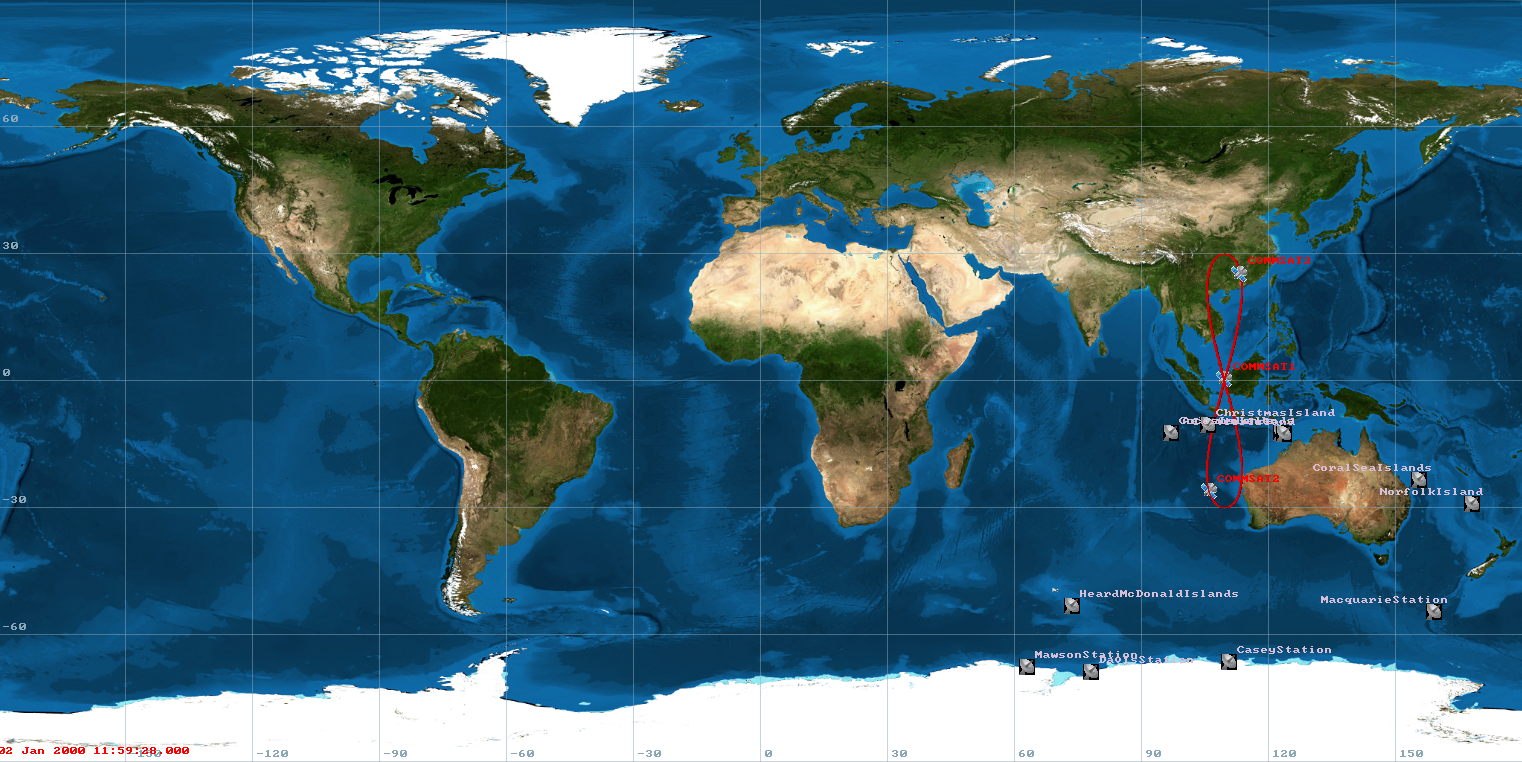
\includegraphics[width=\linewidth]{figures/GroundTrack.png}\\
    \caption{Ground track of constellation over a sidereal day}
    \label{fig:ground_track}
\end{figure}
\begin{figure}[H]
    \centering
    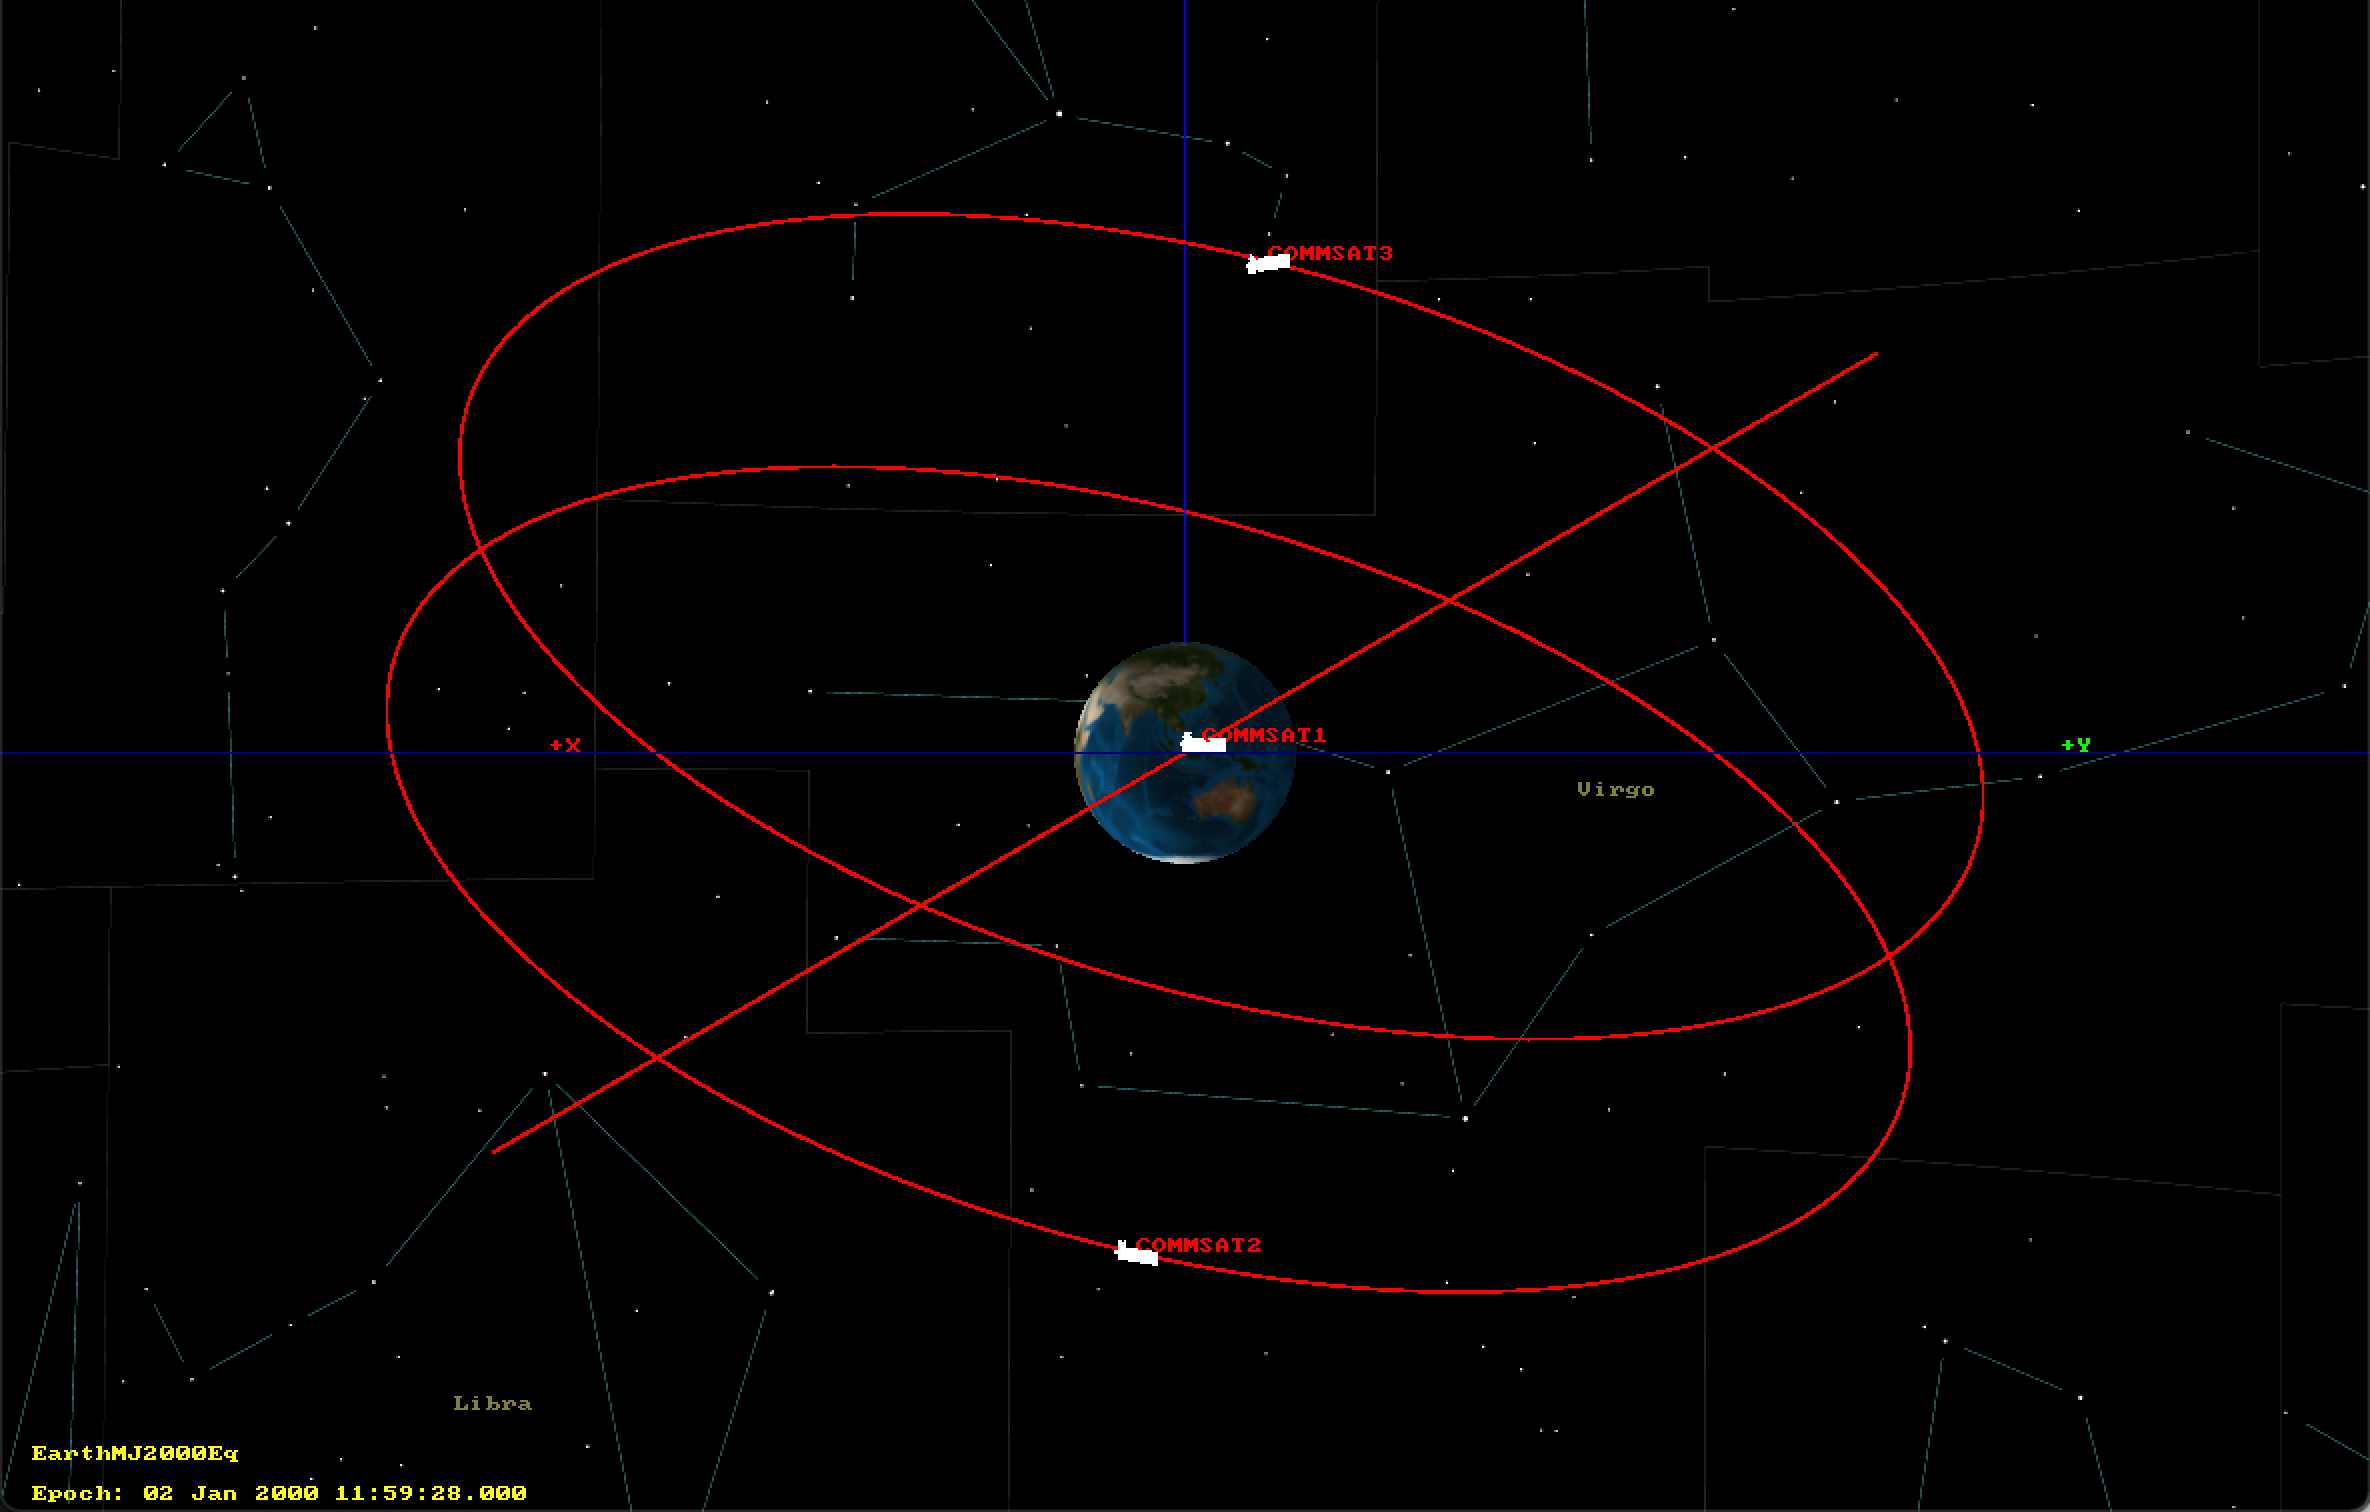
\includegraphics[width=\linewidth]{figures/J2000XY.png}\\
    \caption{Constellation orbits over a sidereal day in the J2000 reference frame, showing the Earth's XY plane}
    \label{fig:j2000_xy}
\end{figure}
\begin{figure}[H]
    \centering
    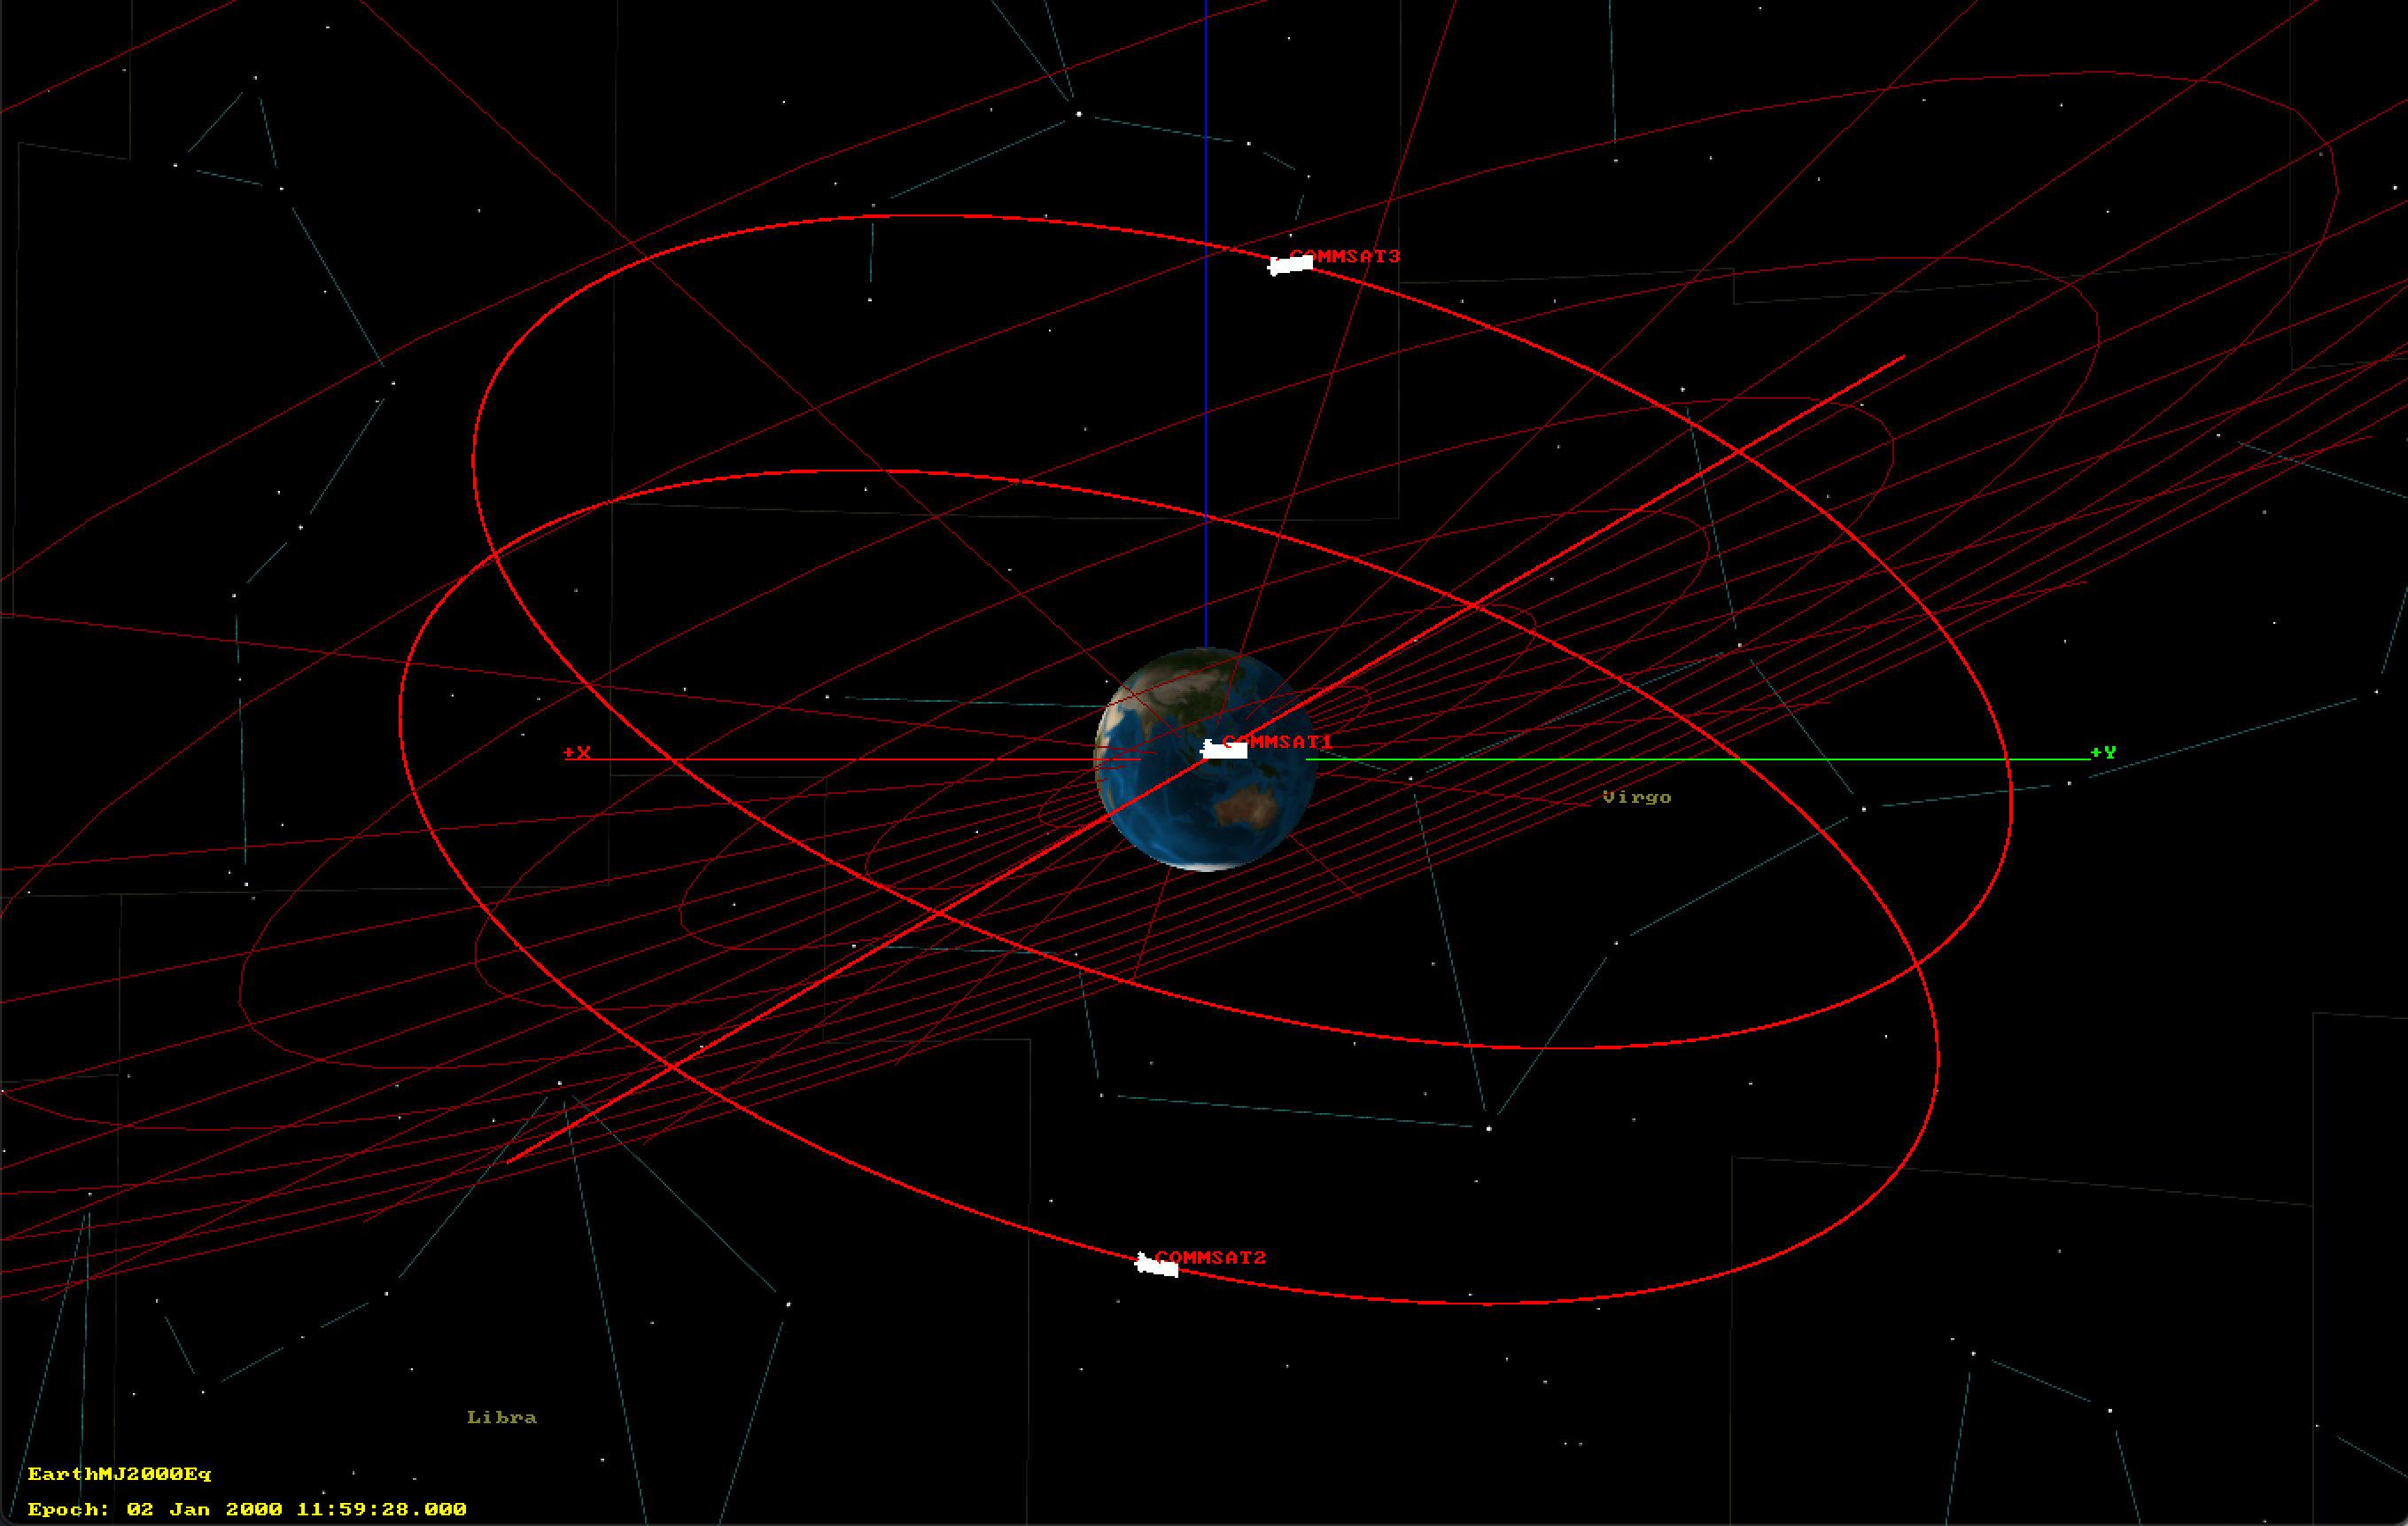
\includegraphics[width=\linewidth]{figures/J2000Ecliptic.png}\\
    \caption{Constellation orbits over a sidereal day in the J2000 reference frame, showing the Earth's ecliptic plane}
    \label{fig:j2000_ecliptic}
\end{figure}
\begin{figure}[H]
    \centering
    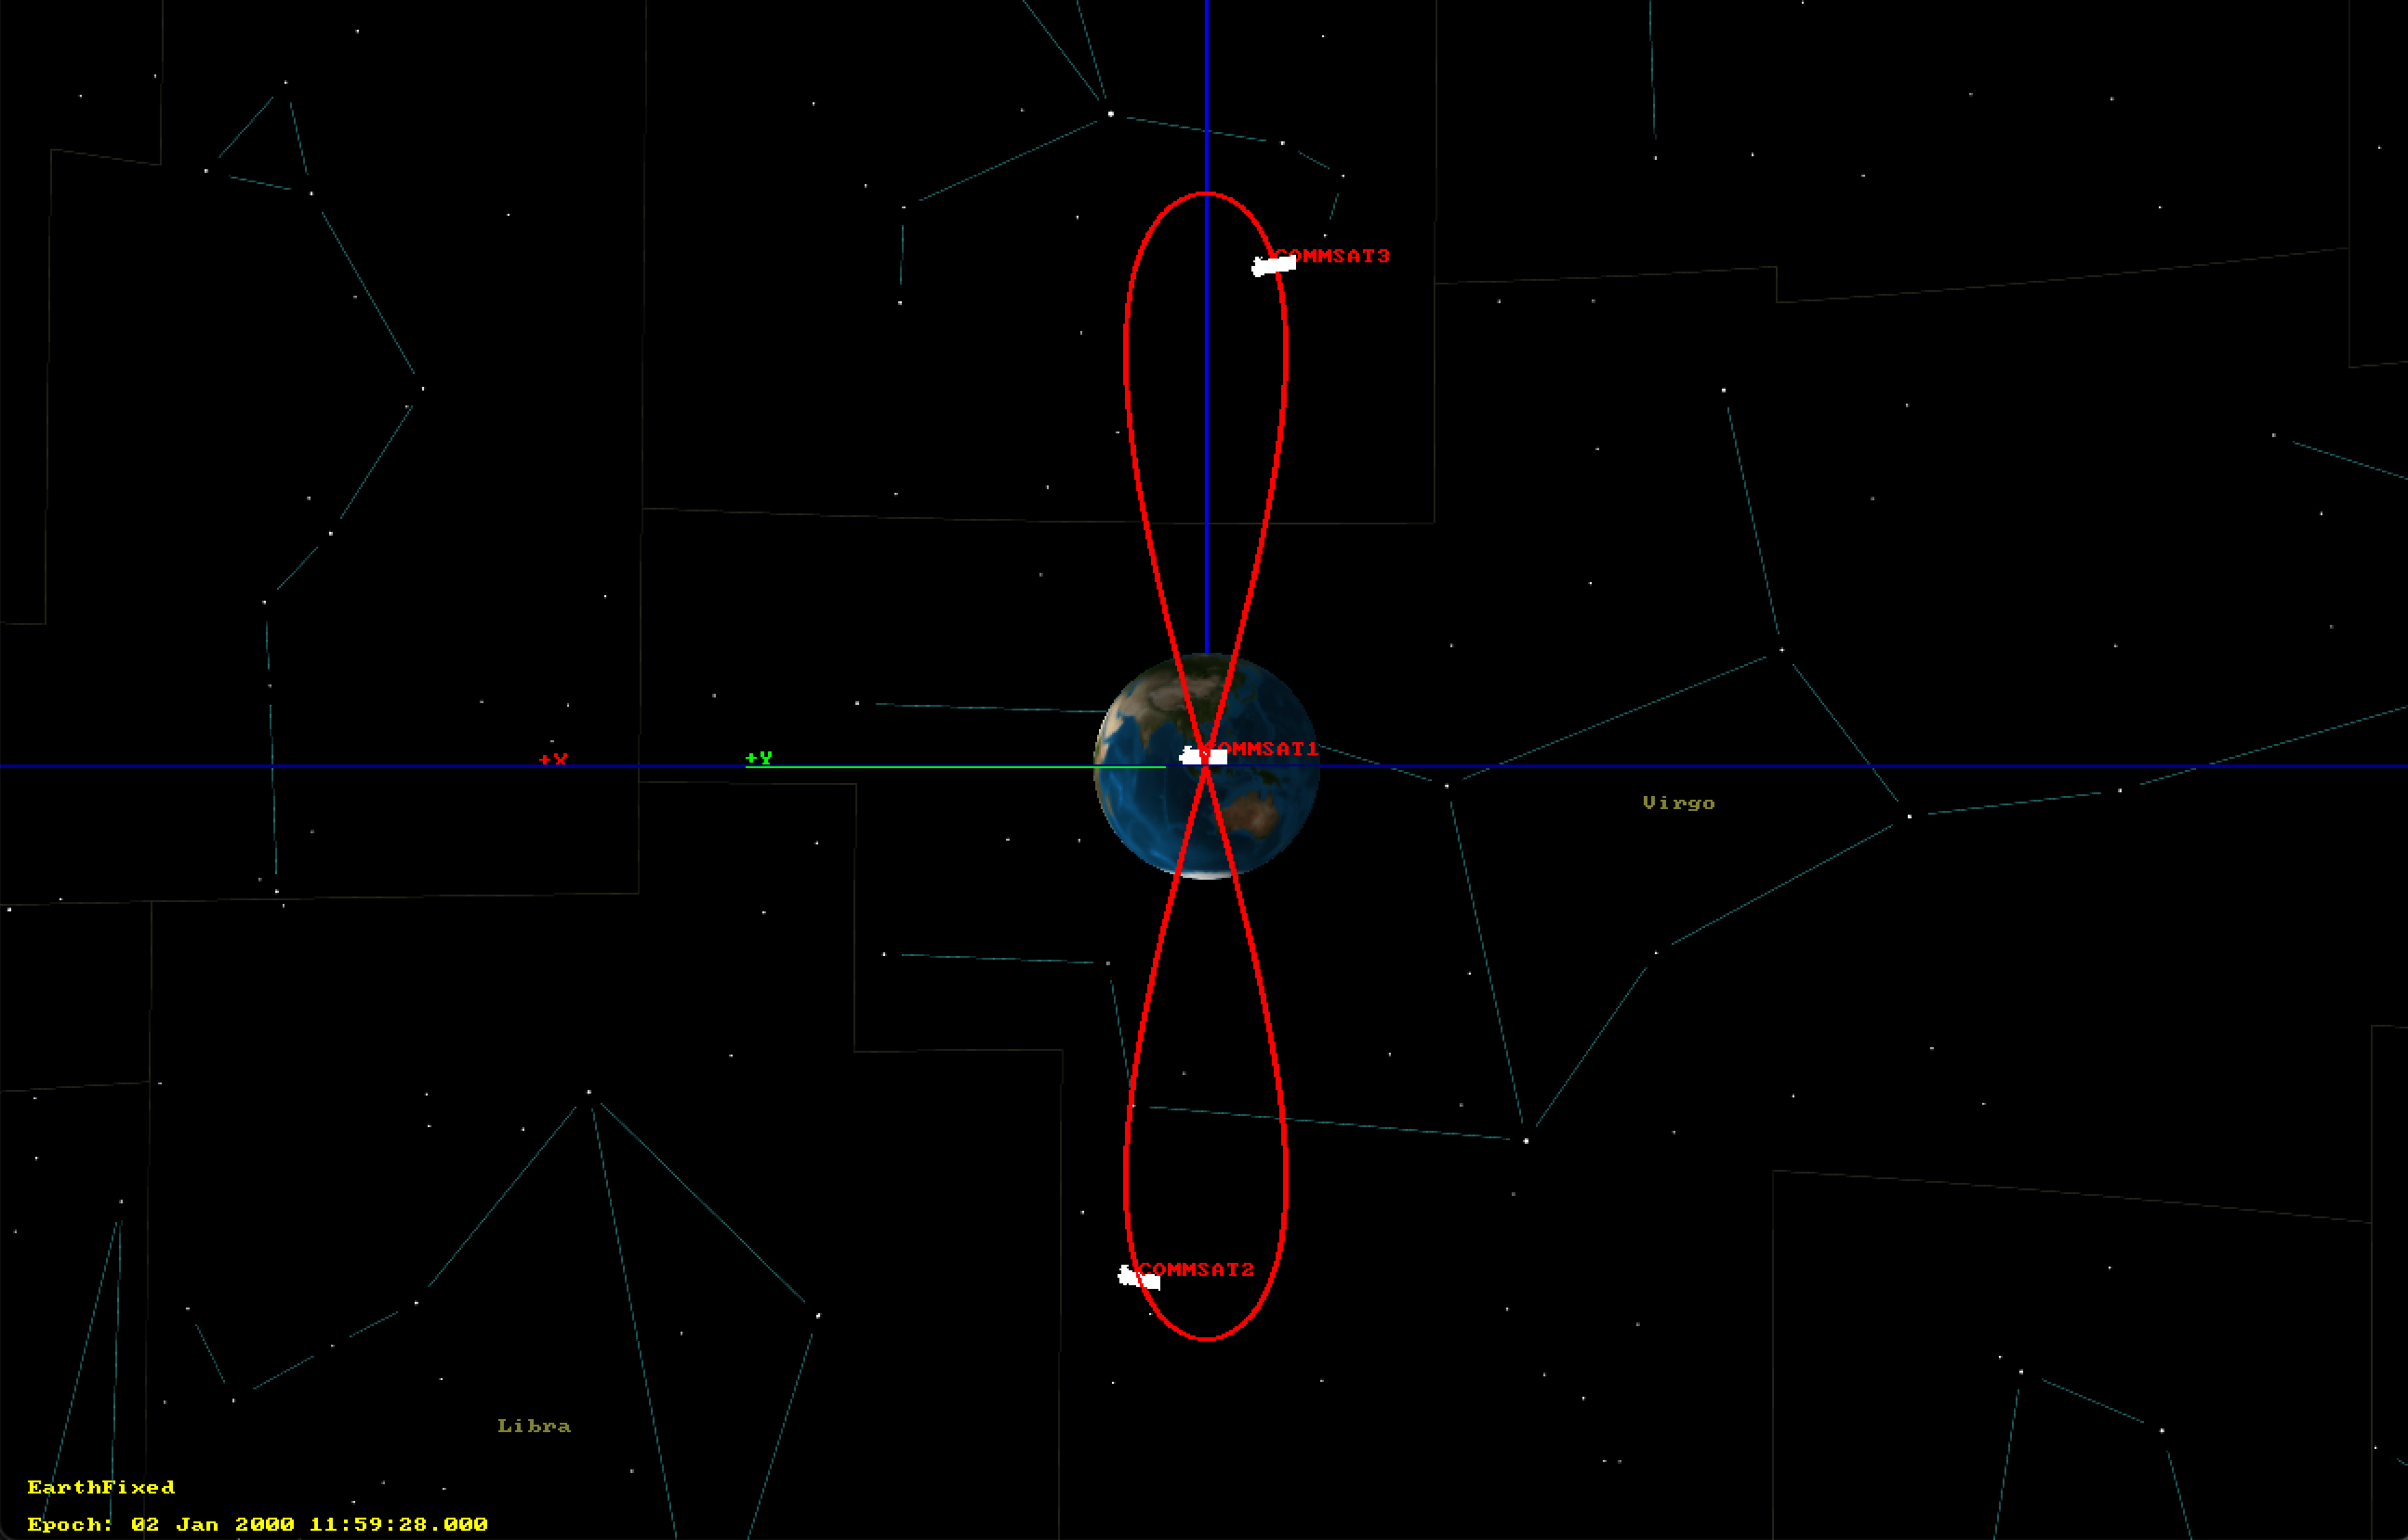
\includegraphics[width=\linewidth]{figures/EarthFixedXY.png}\\
    \caption{Constellation orbits over a sidereal day in the Earth-Fixed reference frame, showing the Earth's XY plane}
    \label{fig:fixed_xy}
\end{figure}
\begin{figure}[H]
    \centering
    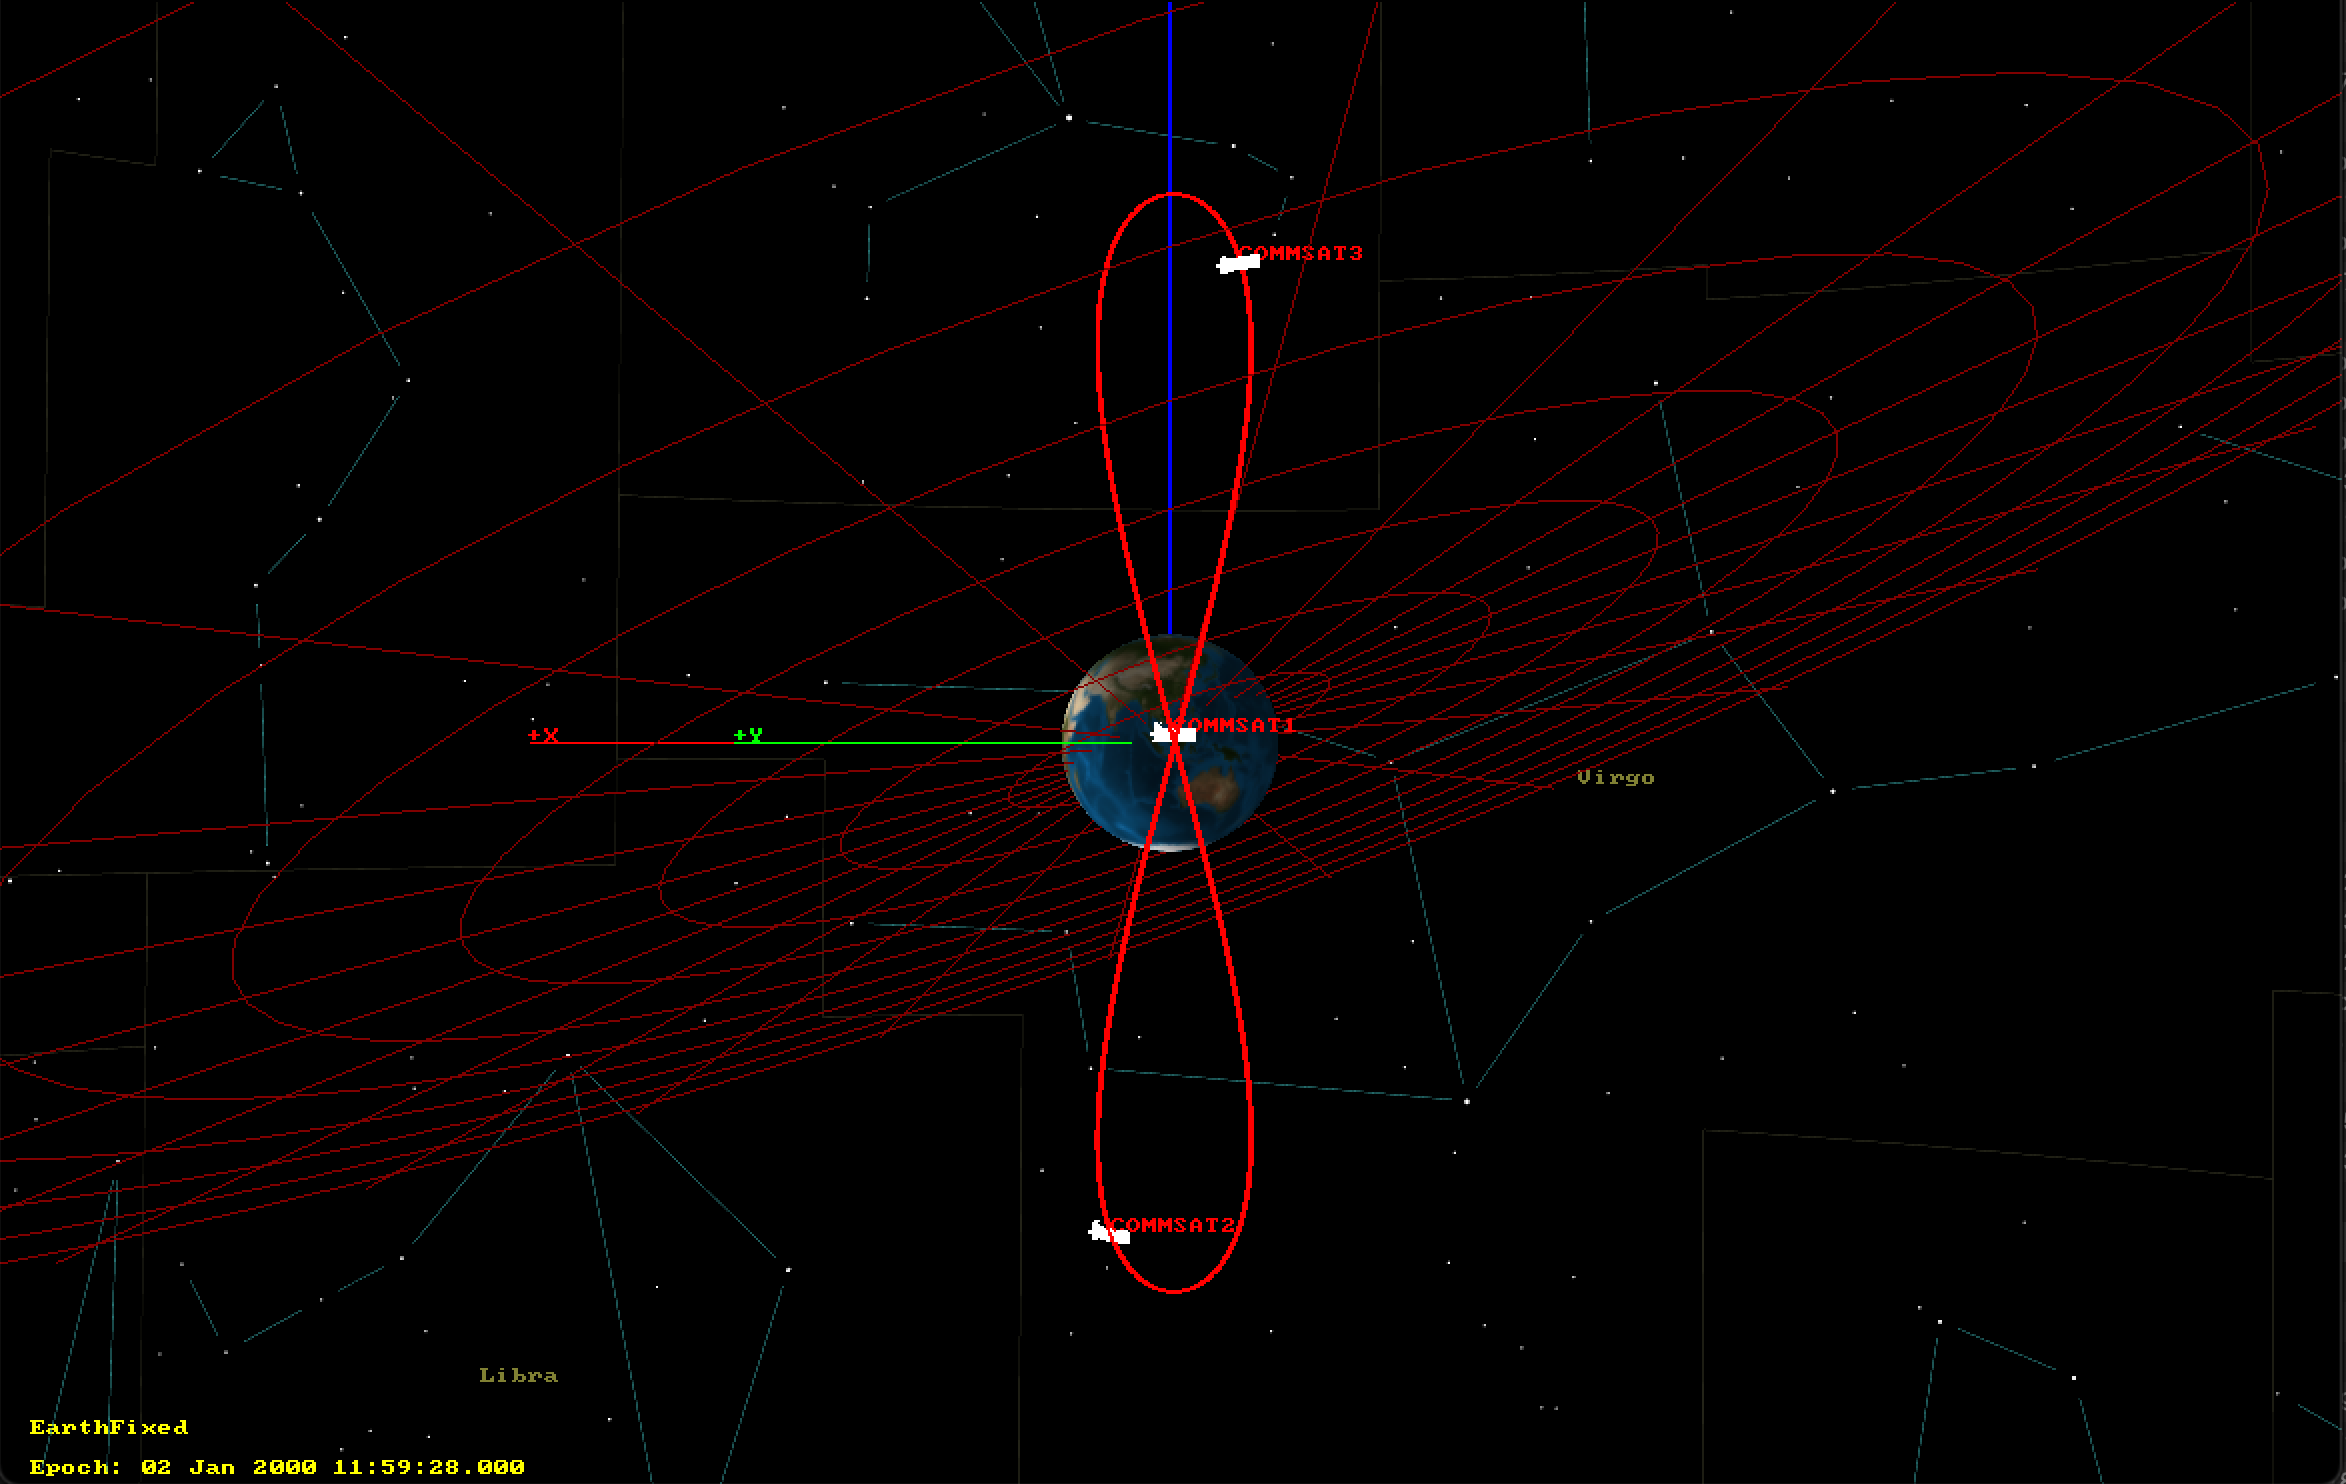
\includegraphics[width=\linewidth]{figures/EarthFixedEcliptic.png}\\
    \caption{Constellation orbits over a sidereal day in the Earth-Fixed reference frame, showing the Earth's ecliptic plane}
    \label{fig:fixed_ecliptic}
\end{figure}
\begin{figure}[H]
    \centering
    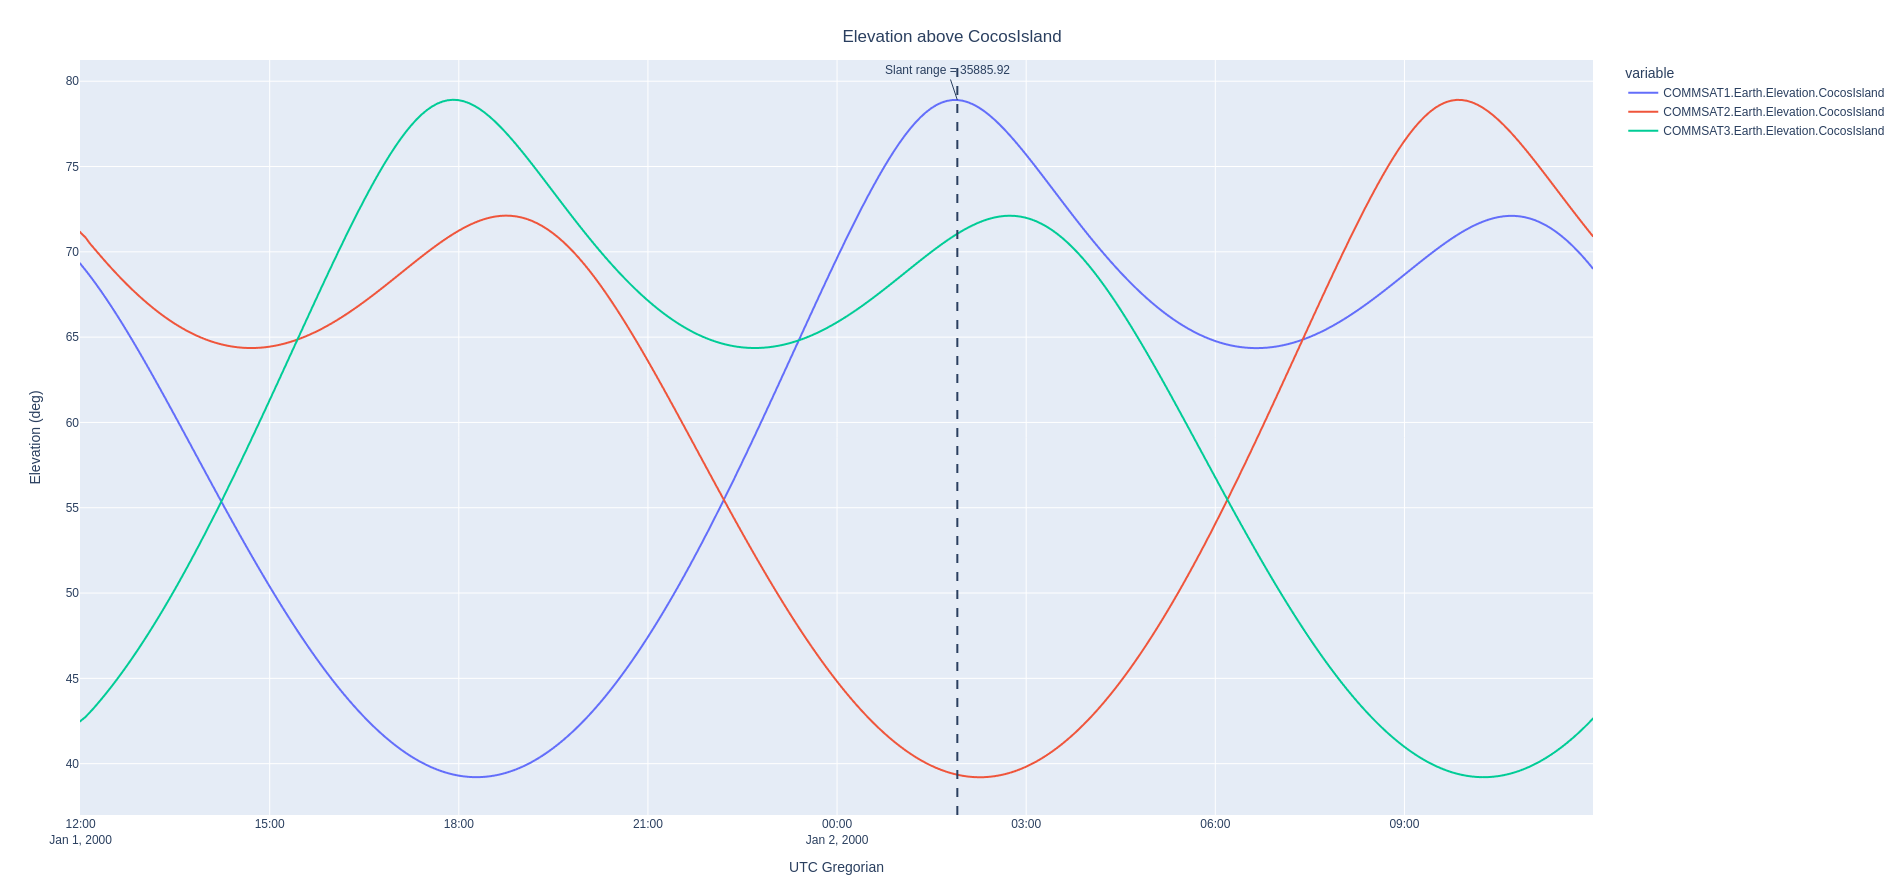
\includegraphics[width=\linewidth]{figures/CocosElevation.png}\\
    \caption{Elevation of constellation over with reference to Cocos (Keeling) Island  over a sidereal day}
    \label{fig:cocos_elevation}
\end{figure}
\begin{figure}[H]
    \centering
    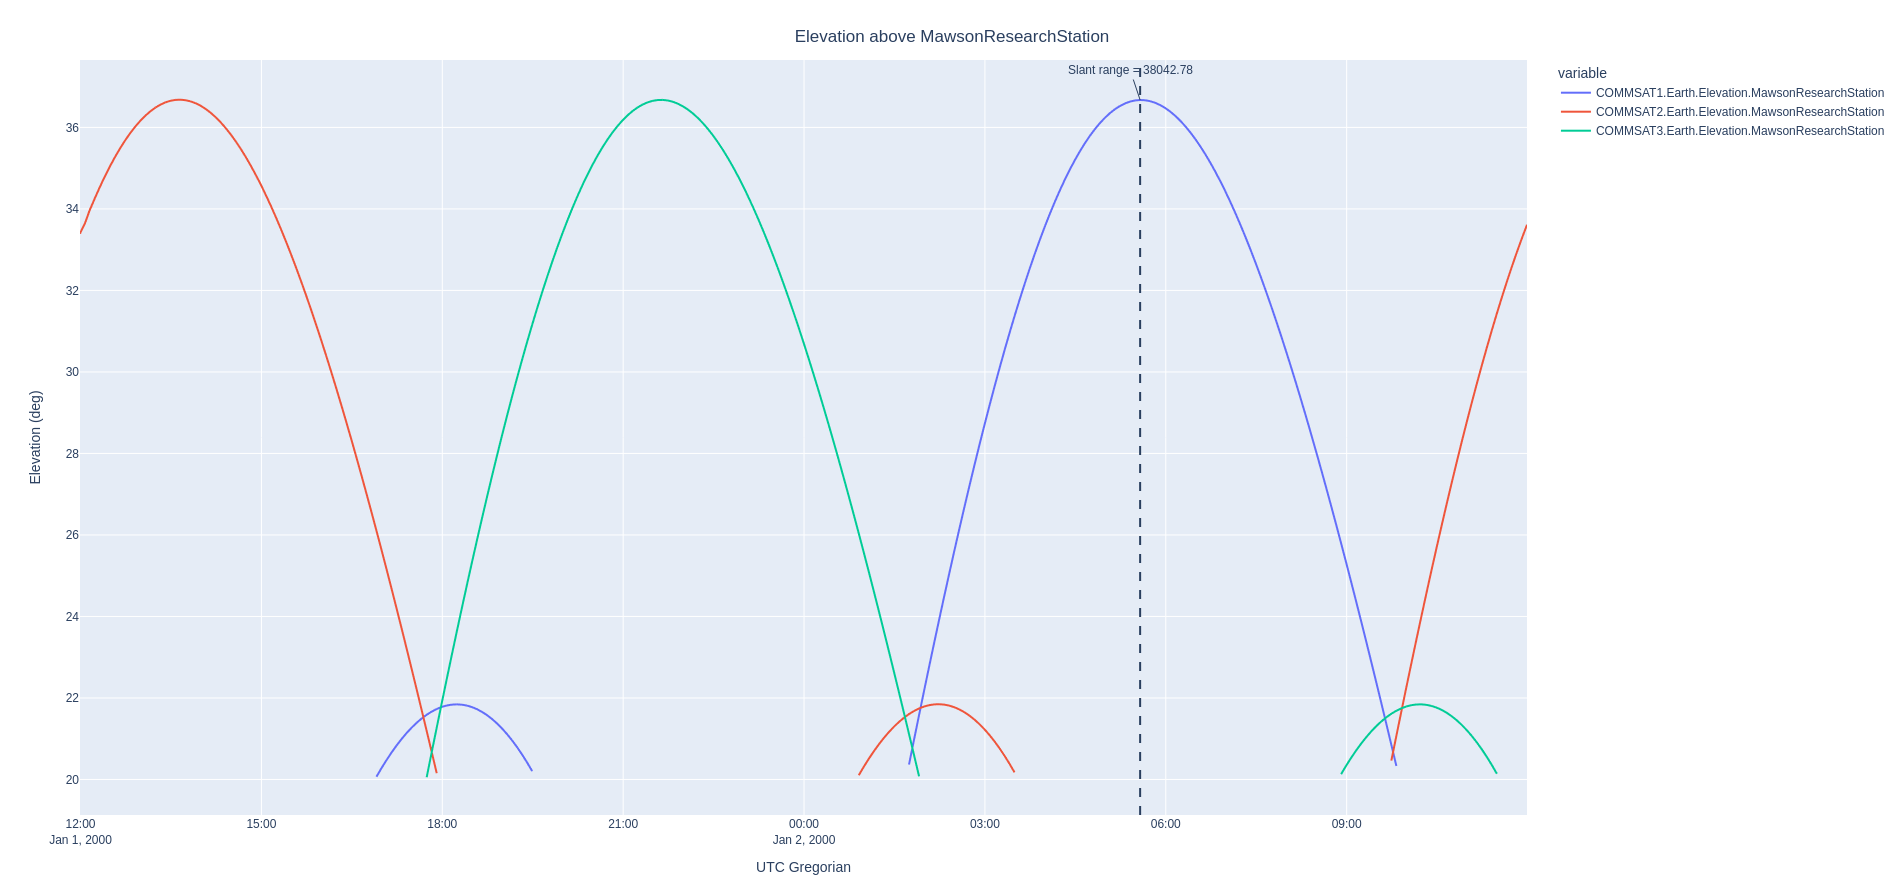
\includegraphics[width=\linewidth]{figures/MawsonElevation.png}\\
    \caption{Elevation of constellation  with reference to Mawson Research Station over a sidereal day}
    \label{fig:mawson_elevation}
\end{figure}
\begin{figure}[H]
    \centering
    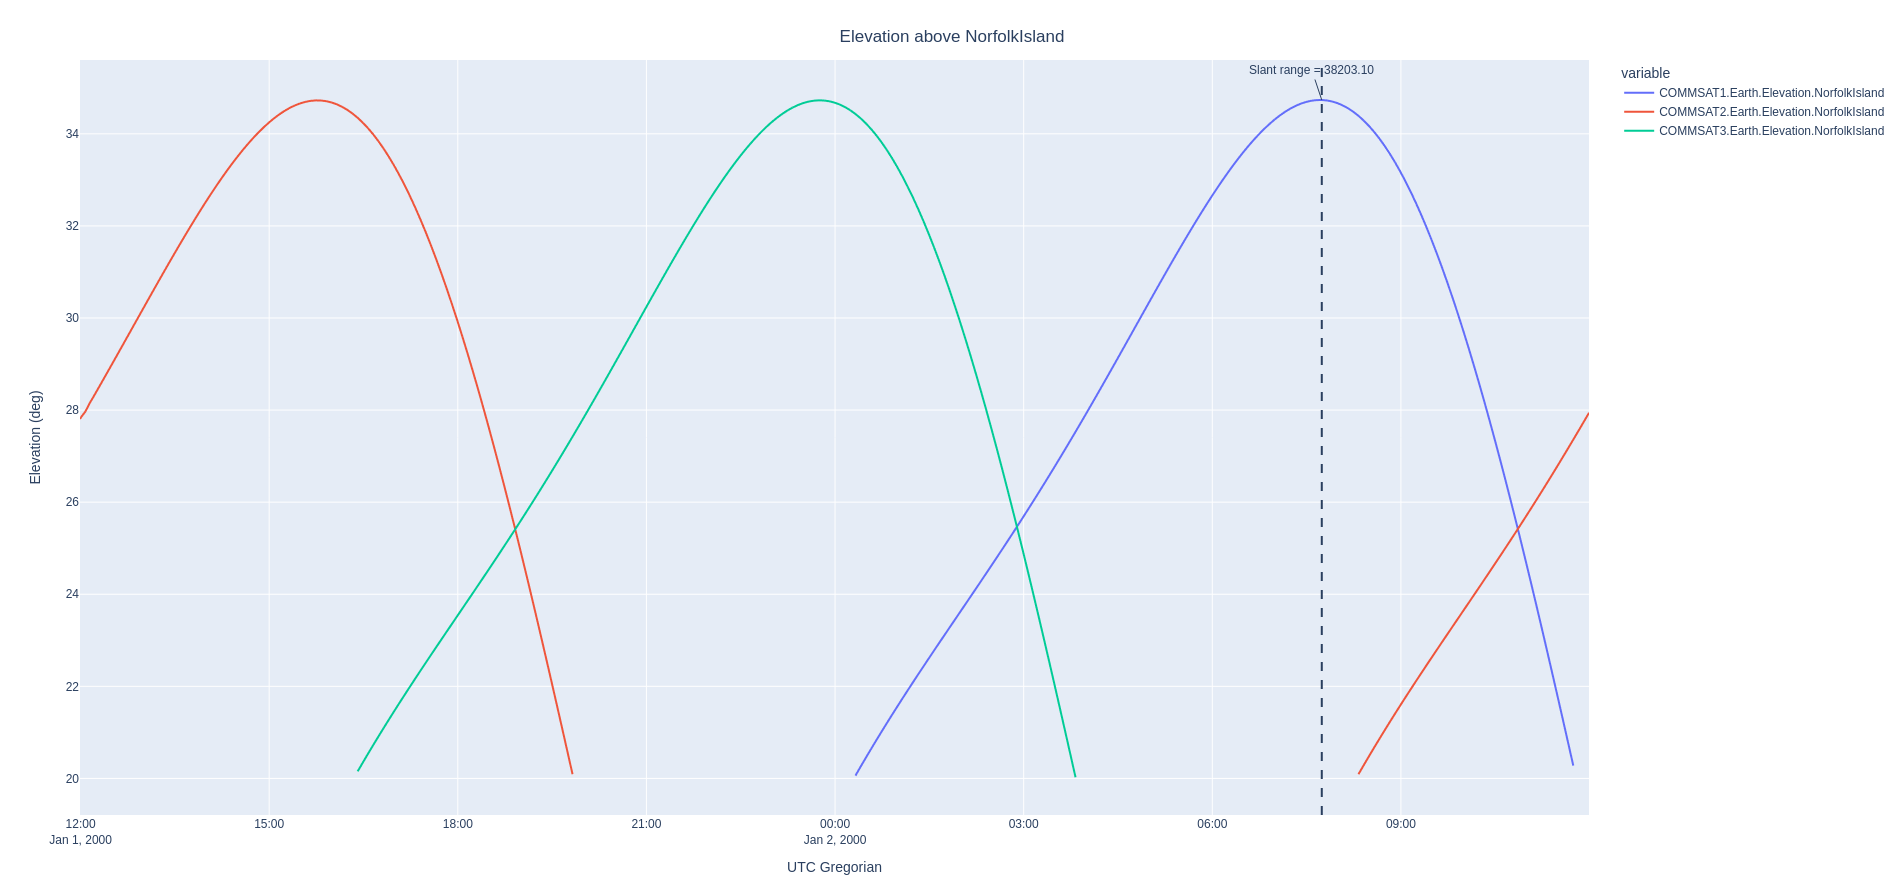
\includegraphics[width=\linewidth]{figures/NorfolkElevation.png}\\
    \caption{Elevation of constellation over with reference to Norfolk Island over a sidereal day}
    \label{fig:norfolk_elevation}
\end{figure}
\begin{figure}[H]
    \centering
    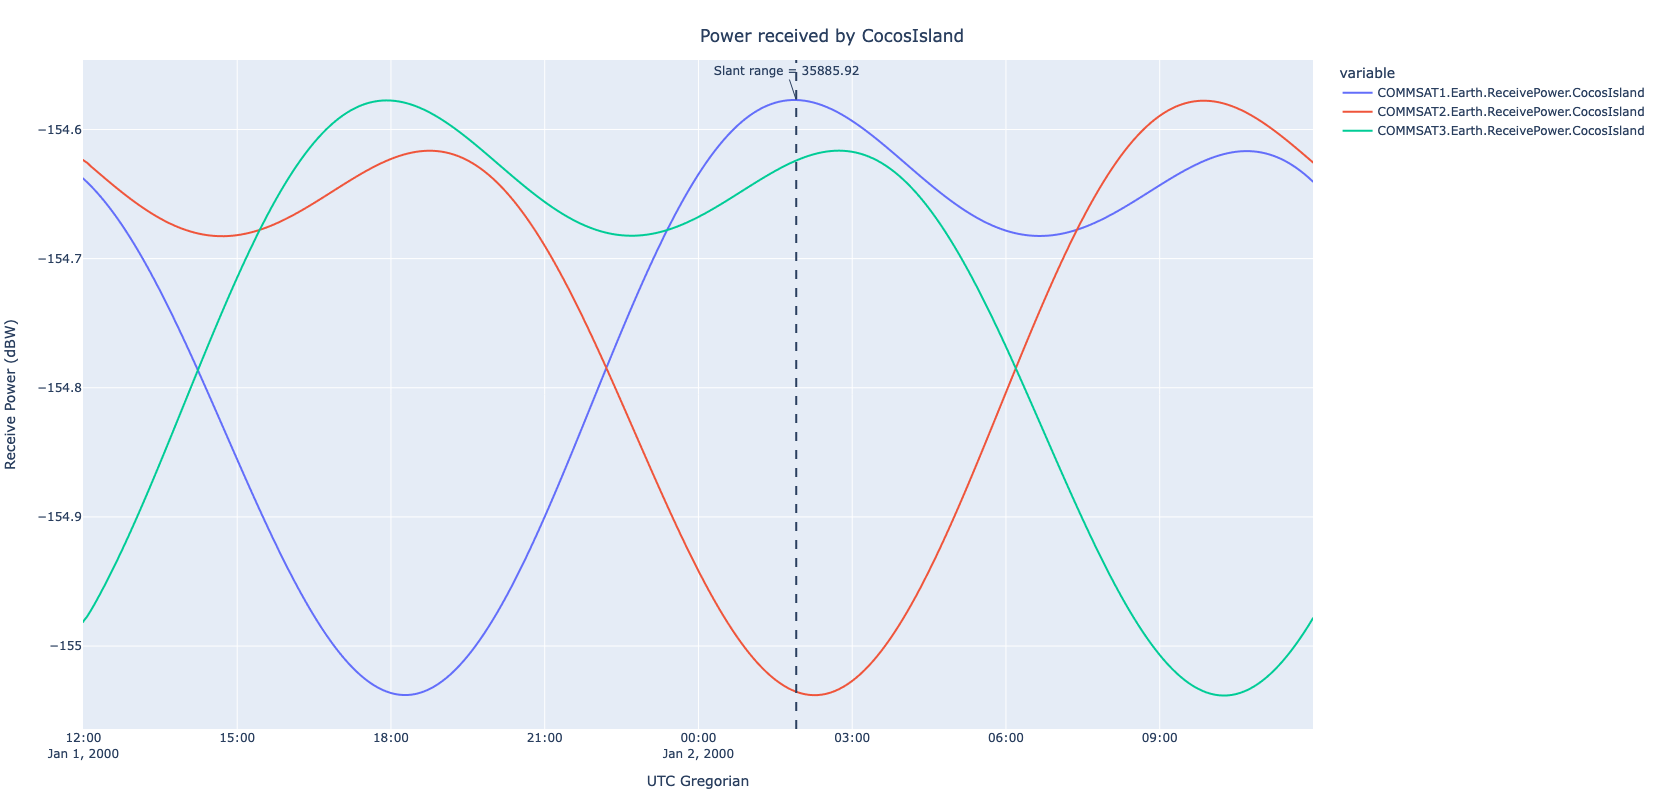
\includegraphics[width=\linewidth]{figures/CocosReceivePower.png}\\
    \caption{Power received at Cocos Island from constellation over a sidereal day}
    \label{fig:cocos_power}
\end{figure}
\begin{figure}[H]
    \centering
    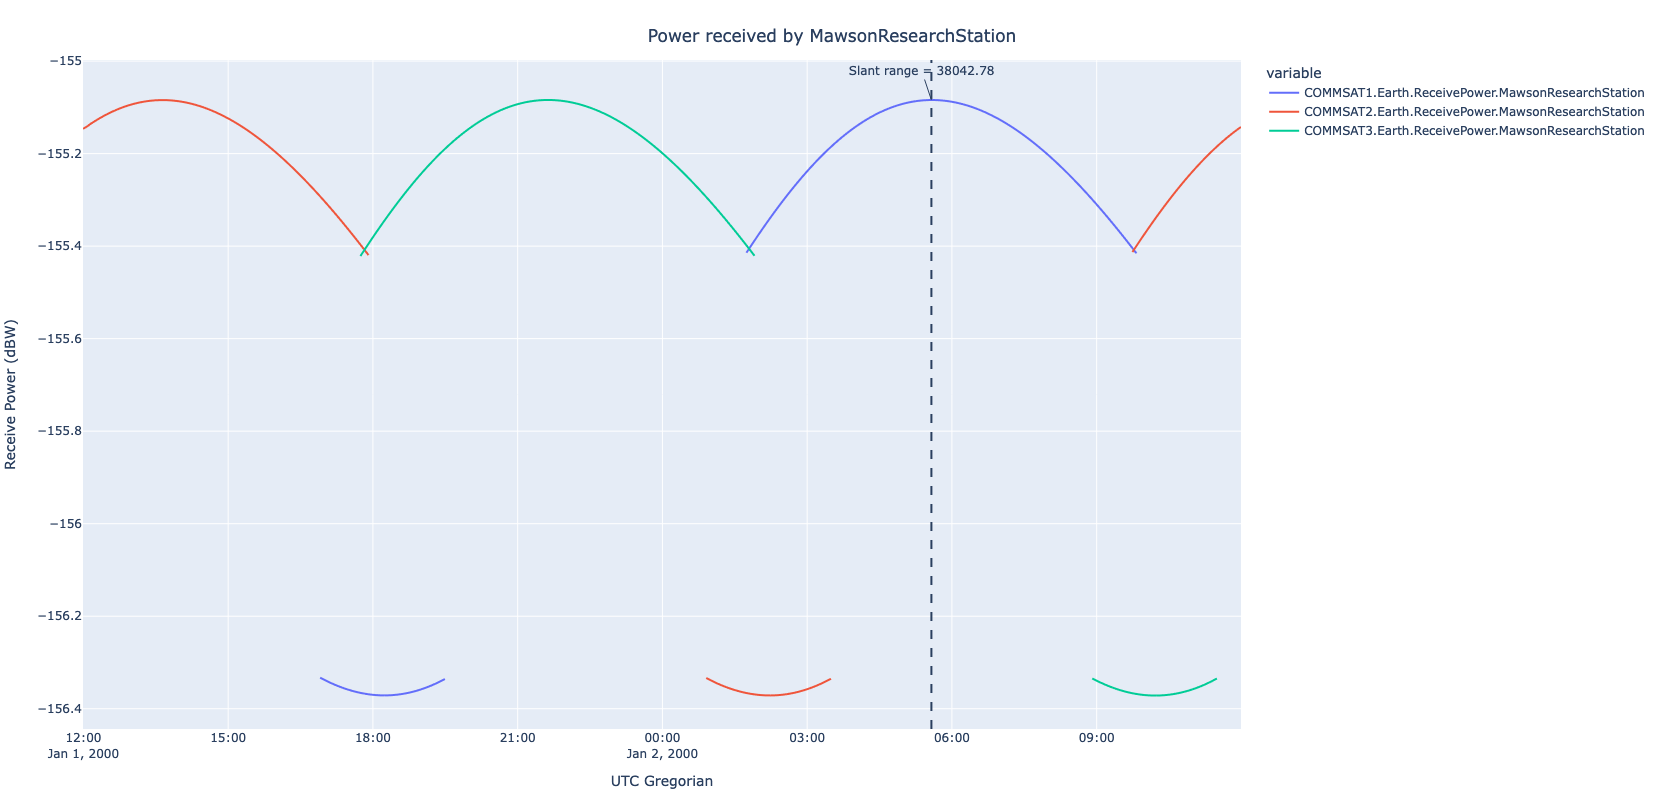
\includegraphics[width=\linewidth]{figures/MawsonReceivePower.png}\\
    \caption{Power received at Mawson Research Station from constellation over a sidereal day}
    \label{fig:mawson_power}
\end{figure}
\begin{figure}[H]
    \centering
    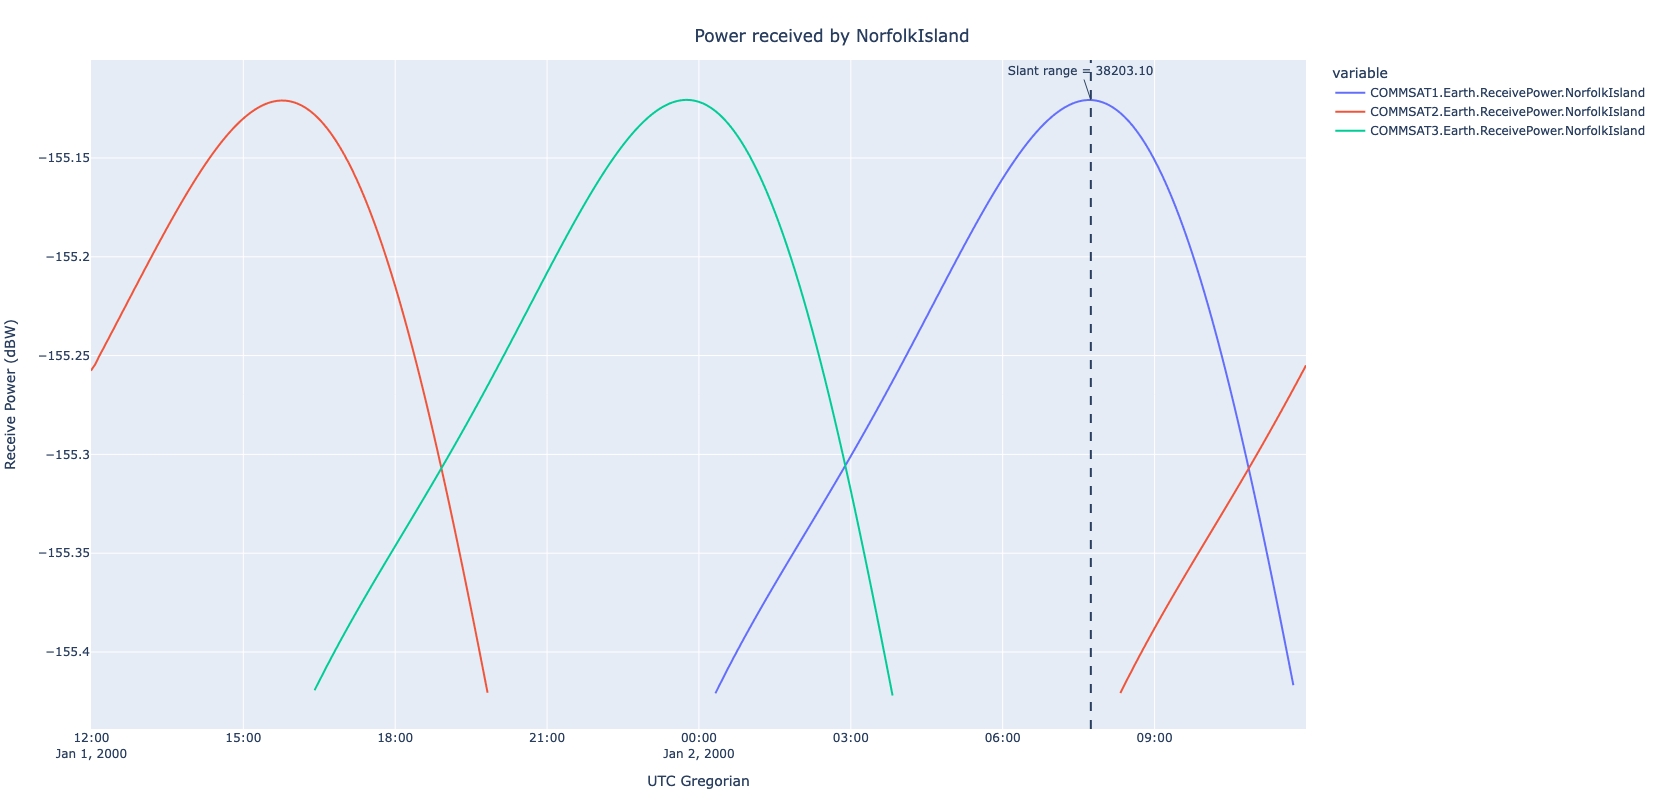
\includegraphics[width=\linewidth]{figures/NorfolkReceivePower.png}\\
    \caption{Power received at Norfolk Island from constellation over a sidereal day}
    \label{fig:norfolk_power}
\end{figure}

\newpage
%=================================================================
%                           List of Figures
%=================================================================
\section{Appendix}
\lhead{Appendix} % section header

\subsection{GMAT Script}
\lstinputlisting[language=Matlab, label={code:gmat}]{code/Assmt1GMATConfig.m}

\subsection{Python Code Samples}
\lstinputlisting[language=Python, caption={main.py}, label={code:main}]{code/assmt1.py}
\lstinputlisting[language=Python, caption={constants.py}, label={code:constants}]{code/constants.py}
\lstinputlisting[language=Python, caption={propagation.py}, label={code:propagation}]{code/propagation_utils.py}
\lstinputlisting[language=Python, caption={orbits.py}, label={code:orbits}]{code/orbit_utils.py}
\lstinputlisting[language=Python, caption={components.py}, label={code:components}]{code/components.py}
\lstinputlisting[language=Python, caption={conversions.py}, label={code:conversions}]{code/conversions.py}

%=================================================================
%                           End Document
%=================================================================
\end{document}